\begin{enumerate}[(a)]
\item \ \\
	
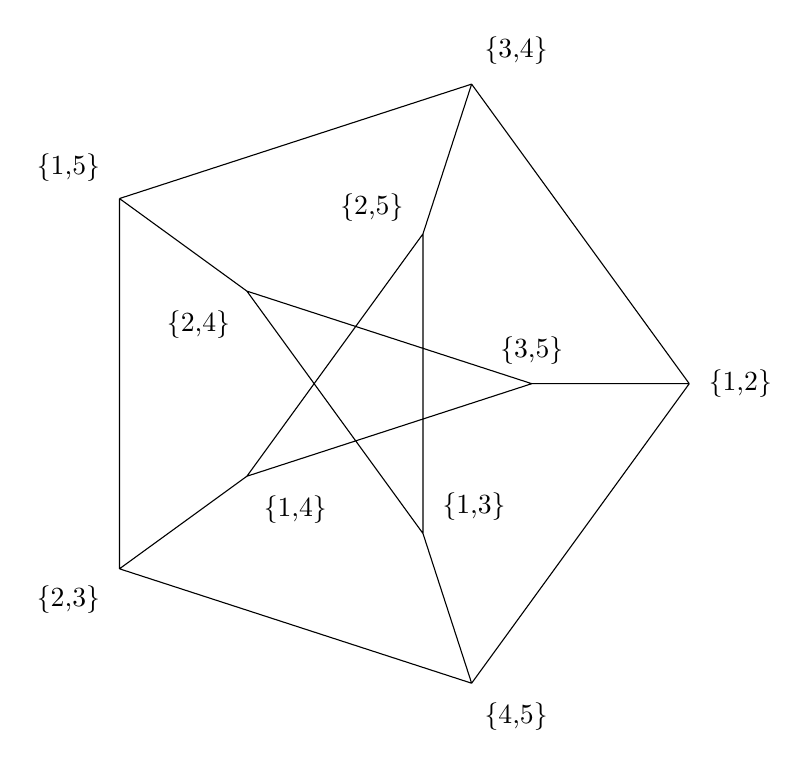
\begin{tikzpicture}
\draw 
(0:2) node [label = {90:\{3,5\}}]{}
(72:2) node [label = {162:\{2,5\}}]{}
(144:2) node [label = {234:\{2,4\}}]{}
(216:2) node [label = {306:\{1,4\}}]{}
(288:2) node [label = {18:\{1,3\}}]{}
(0:4) node [label = {0:\{1,2\}}]{}
(72:4) node [label = {72:\{3,4\}}]{}
(144:4) node [label = {144:\{1,5\}}]{}
(216:4) node [label = {216:\{2,3\}}]{}
(288:4) node [label = {288:\{4,5\}}]{}
\foreach \x in {0,1,...,4} 
{
	(72*\x:2) -- (72*\x:4)
	(72*\x:4) -- (72*\x+72:4)
	(72*\x:2) -- (72*\x+144:2)
};
\end{tikzpicture}

\item The order of $J(n,k,r)$ is just the number of $k$ element subsets of $n$
	elements, or ${n \choose k}$.

\item Let $A$ be a $k$ element subset of $S$. In order to prove that 
	$J(n,k,r)$ is regular, we need show that the number of neighbours of $A$ in
	$J(n,k,r)$ is independent of $A$. But a neighbour of $r$ consists of $r$ vertices
	from $A$ and $k-r$ vertices from $S-A$. We can choose the $r$ vertices of $A$ in
	${k \choose r}$ ways and the $k-r$ vertices of $S-A$ in ${{n-k} \choose {k-r}}$ ways.
	This means the degree of $A$ is ${k \choose r}{{n-k} \choose {k-r}}$, and $J(n,k,r)$
	is regular. By the first
	theorem of graph theory, the size of $J(n,k,r)$ is then just 
	\begin{eqnarray*}
		\frac{1}{2}{n \choose k}{k \choose r}{{n-k} \choose {k-r}} &=& 
		\frac{n!k!(n-k)!}{2k!(n-k)!r!(k-r)!^2(n-2k+r)!}\\
		&=& \frac{n!}{2r!(n-2k+r)!(k-r)!^2}
	\end{eqnarray*}
	if the appropriate binomial coefficients are nonzero. If they are zero (ie when
	$n-k<k-r$) then the graph is completely disconnected.

\item The Petersen graph can be constructed 
	as the complement of the line graph of $K_5$ \cite{petersenwiki}.
	But if the two-element sets making up the vertices of $J(5,2,0)$ are considered
	as edges in $K_5$, then it can be seen that two of them are connected iff they
	are not incident with the same vertex, that is to say
	that $J(5,2,0)$ is precisely the complement
	of the line graph of $K_5$ and hence isomorphic to the Petersen graph.
\end{enumerate}
